\begin{itemize}
    \item [***] \textcite{buenodemesquitaPrinciplesInternationalPolitics2013}{ Chapter 6}
    \item \textcite{allisonConceptualModelsCuban1969}
    \item \textcite{buenodemesquitaDomesticExplanationsInternational2012}
    \item \textcite{putnamDiplomacyDomesticPolitics1988}
    \item \textcite{bendorRethinkingAllisonsModels1992}
\end{itemize}

\section{Bueno de Mesquita, 2013 Chapter 6, Domestic Theories of War}

\begin{enumerate}
    \item War is correctly viewed as ex post inefficient from the perspective of national welfare; however, it can be efficient for leaders, especially those who head a small-coalition, autocratic government.

    \item When domestic politics plays a part in shaping demands for war, it can increase the credibility of threats, reduce the likelihood of threats, and alter the path of conflict escalation.

    \item Domestic politics alter the subject matter of war. Domestic accountability makes the pursuit of policy concessions and regime change focal issues for democracies. In autocracies, the focal issues for which wars are fought involve resource acquisition and territorial conquest.

    \item Democrats try harder to win the wars they fight than do autocracies, and democracies are more selective about their preparedness to fight. Selection effects identified by examining domestic politics fundamentally alter the trajectory of conflict from what is expected if we take the view that states are unitary actors.

    \item Weakness, a characteristic of terrorists and of many small states, may encourage otherwise peacefully inclined people to become unusually aggressive because they bring few bargaining chips to the negotiating table.
\end{enumerate}

\subsection{The Domestic Politics of International Crises}
\begin{enumerate}
    \item \textbf{Kosovo (1999):} NATO bombed Serbia to force Milošević to stop the expulsion of the predominantly Muslim Kosovo Albanians. The intervention was not prompted by an existential threat to NATO countries, although the refugees would have imposed a major burden on neighboring states.
    \item \textbf{Bosnia (1995):} Through Operation \textit{Deliberate Force}, NATO intervened to stop Serbia’s involvement in ethnic cleansing in Bosnia. The text presents this as another intervention that cannot be explained solely by national security or the balance of power.
\end{enumerate}

Here we have examples in which, as Fearon (1995) suggests, war might be ex post inefficient for the countries involved but, as Chiozza and Goemans (2004) note, war might not be inefficient for the individual leaders choosing between war and the peace of appeasement.

\subsection{Ex-post Efficient War: Falkland Islands}
\begin{enumerate}
    \item Little economic value
    \item Little political value
    \item Possible diplomatic alternative: couple of billion dollars to convice Argentines to not fight
\end{enumerate}
She made a wise decision for her, not for Britain.

Thatcher chose to fight spending a couple billion dollars to defeat Argentina.

Why did this make sense? Thatcher turned her career around by defeating Argentina.

After becoming prime minister in 1979, Thatcher launched a major economic reform in Britain to try to turn its economy around. In the short term, her economic program and her fights with trade unions led to recession and high unemployment. In the wake of the economic downturn, she became extremely unpopular.

Autocrats are much less sensitive to military defeat.

\subsection{Audience Costs: Cuban Missile Crisis}
The planning for the invasion Kennedy backed the invasion but withheld American air cover, which had been promised to the Cuban ex-patriots who led the landing on Cuba. The invasion was a total failure.

This and President Kennedy’s weak performance at a summit meeting with Khrushchev convinced the Soviet leadership both that Kennedy could be pushed around and that they could place offensive nuclear missiles on Cuba.

\begin{itemize}
    \item \textbf{September 1962:} The Soviets began deploying nuclear-armed missiles in Cuba. However, these missiles did not fundamentally alter the balance of power.

    \item \textbf{October 14:} The Soviet buildup of an offensive capability was discovered, leading the United States to impose a naval quarantine of Cuba.

    \item \textbf{October 24:} Soviet ships stopped short of the quarantine line rather than confront the US Navy. As we now know, the Soviets had nuclear-armed submarines available in case of a confrontation.

    \item \textbf{Between October 24 and 27:} Khrushchev sent a private letter to Kennedy stating that the Soviet Union's need for weapons in Cuba would disappear if the US government pledged not to invade the island.

    \item \textbf{October 27:} Khrushchev's private letter was followed by a public demand that the United States remove its offensive missiles from Turkey.

    President Kennedy responded to the first, private message by demanding that the missiles in Cuba be made immediately inoperable.

    Privately Robert Kennedy informed the Soviet leadership that the United States would remove its missiles from Turkey in the future.

    \item \textbf{October 28:} Premier Khrushchev publicly announced that the USSR would withdraw its missiles from Cuba.
\end{itemize}

The missiles on Cuba had not fundamentally altered the balance of power.

The president
\begin{enumerate}
    \item Was concerned that if he did not take strong action he would be impeached.
    \item mid-term elections were only a few short weeks away.
\end{enumerate}

The public declarations that Kennedy made are examples of what James Fearon (1994) calls audience costs.

Kennedy had a domestic price to pay if he backed down after making public threats about an (unexpected) offensive weapons buildup on Cuba.

According to the model, high audience costs make it hard for democratic leaders to back down after a severe public declaration such as Kennedy made. We will also see that the difficulty in backing down can make crises less likely to occur and can make nondemocratic adversaries more likely to back down themselves if they are threatened.


\subsection{Model}

\begin{center}
    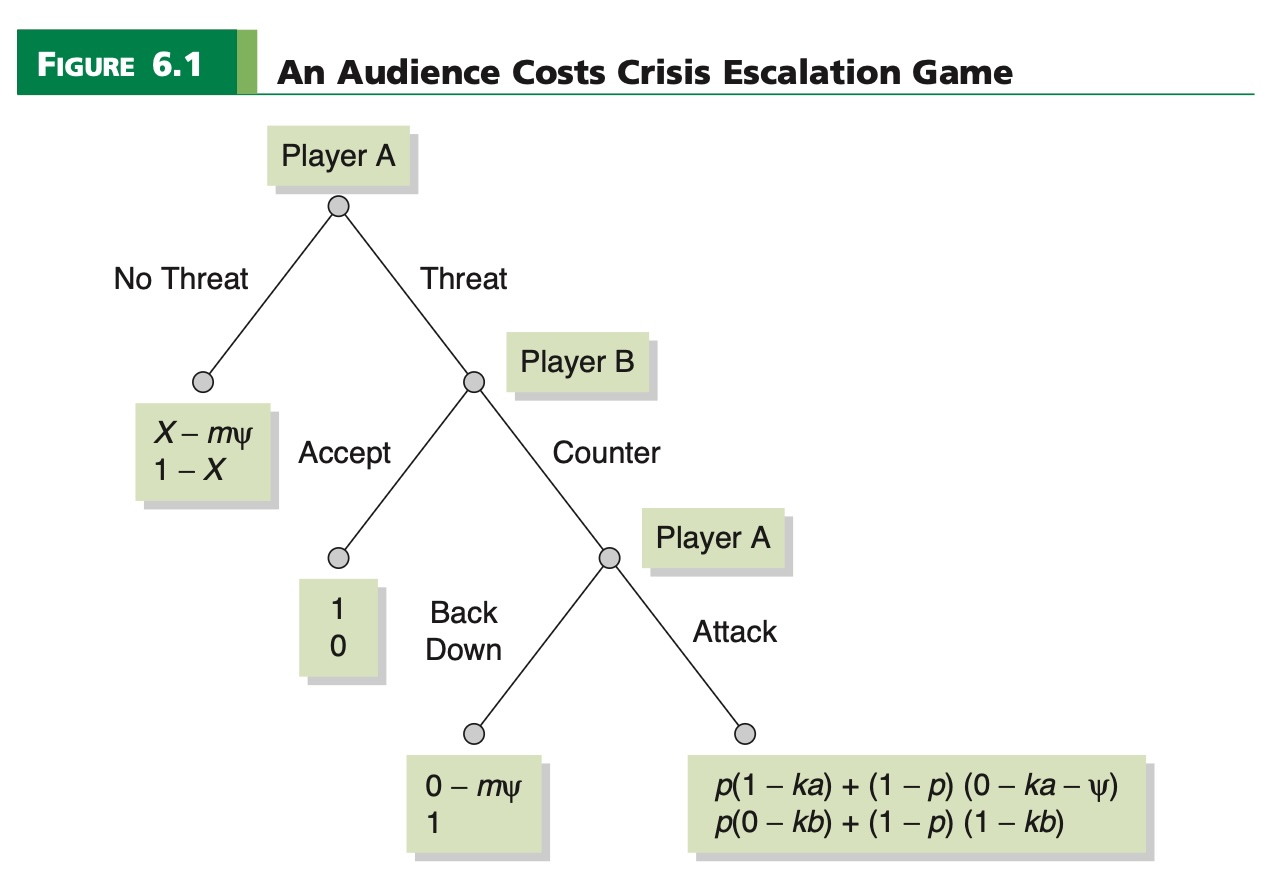
\includegraphics[width=0.7\textwidth]{images/audience_costs_crisis_escalation_game.jpg}
    \captionof{figure}{\label{fig:fig8_audience_costs_crisis_escalation_game.jpg}%\textit{\parencite[Fig.\(\backsim\)1]{cranmerWhatCanWe2017}}
    }
\end{center}

\begin{itemize}
    \item Let $0 \leq m \leq 1$: the variable $m$ measures the degree of domestic policy inadequacy (the general risk of not being reselected) based on prior job performance.

    \item $\Psi$ is the cost to a leader of being turned out of office: a constituency- or audience-imposed cost.

    It measures the audience costs associated with the leader’s choices in the game since loss of office is the cost the selectorate can impose on a leader who fails to deliver the benefits they seek.

    \item $X$ is the value of the status quo to player A.

    \item $p$ is the probability that A wins if A attacks B.

    \item $k_a$ and $k_b$ are A's and B's expected costs from war.

    \item Assumptions: winning a war or making a successful threat ensures remaining in office. Losing a war ensures losing office. Backing down after threatening war or not threatening war implies that the loss of office depends on the degree to which the leader's record is considered inadequate ($m$).
\end{itemize}

% In this game, A’s possible strategies are:
% \begin{enumerate}
%     \item [(1)] threaten and attack;
%     \item [(2)] threaten and back down (bluff)
%     \item [(3)] not threaten and attack: this strategy is eliminated by the rules for calculating a subgame
%     perfect Nash equilibrium
%     \item [(4)] not threaten and back down.
% \end{enumerate}

% In this game, B’s possible strategies are:
% \begin{enumerate}
%     \item [(1)] counter A’s demand
%     \item [(2)] accept A’s demand
% \end{enumerate}

$\Psi\ \text{and}\ m$ are both domestic features in the crisis decision-making game and so \textbf{are not part of a realist perspective}.

\subsubsection{Solving when $\Psi = 0$ and $m = 0$}
Backward induction reveals that A will attack rather than back down if A has threatened and if $p > k_a$.

B can be expected to counter under two circumstances:
\begin{enumerate}
    \item [(1)] if A is expected to back down (B believes $p < k_a$)
    \item [(2)] if B believes A will attack but B believes that $1 - p > k_b = $ B’s expected chance of winning $1 - p >$ B’s expected costs from a war ($k_b$).
\end{enumerate}

A initiates a threat only if:
\[A\ believes\ that\ B\ believes\ 1 - p < k_b\]
\[B\ will\ not\ counter\]
\[A\ believes X + k_a < p\]
\[\text{X is so bad that it is worth gambling on a war}\]

In each instance, we see that:
\[p\ \uparrow\ \Rightarrow\ \uparrow\ Probability\ A\ makes\ a\ threat\]
\[p\ \uparrow\ \Rightarrow\ \uparrow\ \text{threaten and
more likely to fight if B makes a counter demand instead of backing down}\]

\subsubsection{Solving when $\Psi > 0$}
Holding everything else constant, increased audience costs
changes the size of the fraction that $p$ must be larger than in order to attack rather than back
down.

If $m$ is sufficiently large, then the leader of A is prepared to attack even with a small chance of winning as this is its best shot at salvaging his or her reelection prospects.

So good prior policy performance can offset the incentive to attack even when audience costs are high.

We learn from audience costs two important things: each pulling in opposite directions with regard to settling disputes.

\begin{itemize}
    \item that democrats are less likely to make idle threats
    \item democrats might attack even when their chances of victory are low
\end{itemize}

\subsection{Crisis Selection in Democracies and Autocracies}
As Schultz (1998, 2001) has noted, audience costs lead to interesting selection effects in terms of what we actually get to observe in the world.

A legitimate opposition is absent from audience-costs models.

In Schultz’s formulation
\begin{itemize}
    \item because the opposition party is interested in gaining electoral advantage, it opposes foreign policies the incumbent proposes if the opposition deems the policy likely to fail.
    \item When the foreign policy is thought to have a good chance of success, the democratic opposition backs it to minimize the electoral advantage gained by the incumbent’s party.
\end{itemize}

When the opposition supports the incumbent’s foreign policy, this support credibly conveys “high resolve” to the foreign opponent. This has two effects: (1) it encourages the democratic incumbent to press ahead with his foreign policy and (2) it discourages the rival from believing that internal dissension in the democracy will weaken the democratic leader’s resolve to fight.

The audience-costs literature offers an explanation for differences in the crisis behavior of autocrats and democrats. It helps us understand selection effects that shape what we actually observe in the international arena.

\subsection{Diversionary War}
Smith (1996, 1998) developping a model in which audience costs are an endogenous, strategic element of the political environment.

In Smith’s model, leaders can use their private information to manipulate policy, choosing, for instance, diversionary war tactics designed to draw attention away from their previous policy failures (the variable m in the game in figure 6.1). Other models, such as those by Slantchev (2006) and Ashworth and Ramsay (2011) further develop these themes.

In the Ashworth-Ramsay model, for instance, leaders have private information about their nation’s prospects in war (p in figure 6.1). That information can be used to extract a substantial concession from the foreign rival who wishes to avoid the costs of war (kb). But the fact that the initiation of conflict could extract a significant concession to appease the initiator means that the prospective initiator also has incentives to create a crisis when her private information does not support a strong expectation of victory.

Ashworth and Ramsay report that under optimal conditions, citizens always punish leaders if they initiate a crisis and then back down. Whether leaders are punished if they back down rather than going to war, however, depends on the value of the status quo and on the costs of war, much as we saw in the game in figure 6.1.

Gaubatz (1991), Fordham (1998), and Smith (2004), for example, show that war timing by democratic leaders is strongly influenced by where they are in their election cycle, their reelection prospects, and the electoral rules under which they operate.

Conconi, Sahuguet, and Zanardi (2010) show that democratic term limits lift some of the constraints on war fighting that otherwise characterize reelection-motivated choices in democracies.

Morrow focused on arms control negotiations between the United States and the Soviet Union, demonstrating that when the US economy faced high inflation or high unemployment (i.e., m is large in figure 6.1), the president was prepared to grant greater concessions to the powerful Soviet Union in arms control talks to offset his domestic economic shortcomings and to improve the odds of a negotiated resolution of important, contentious foreign policy issues.

Tarar focuses on what makes a diversionary threat into a meaningful signal of leader competence. He argues that the rival must be sufficiently strong that the conflict actually tests competence, and the leader must place a sufficiently high value on retaining office. Tarar’s model helps make sense of seemingly competing empirical patterns.

\subsubsection{The Resurrection Hypothesis - Downs and Rocke (1995)}
When leaders face a military defeat and anticipate being ousted, extreme efforts are actually a rational response.

Such leaders lose nothing by fighting on and stand to gain much if luck should turn their way.

\textbf{Example: Tet Offensive during Vietnam War}
US military and political leaders believed that they had already punished the North Vietnamese regime to such an extent that it was no longer capable of launching a military offensive. Likewise, the American public had become convinced that the war in Vietnam was virtually won. And, in fact, the Tet offensive was a considerable military rout But just by the very fact that they were able to launch the offensive at all, the North Vietnamese pulled off a stunning political and propaganda victory that resurrected their hopes and led, ultimately, to a negotiated resolution of the Vietnam War that was very favorable to the North Vietnamese side.

\textbf{Example: Iraq 2003}
Bluffing about WMD weapons, Saddam might have hoped to convince the opposition in the United States to oppose going to war given the high expected costs in terms of casualties.

Saddam Hussein may have decreased the odds of an invasion by raising the specter of an unconventional war.

When a country demonizes an adversary, this helps mobilize domestic political support for the use of force, thereby increasing the chances of victory against the adversary. However, demonizing an enemy also motivates that adversary to try harder to win.

\subsubsection{Pacific Dove Hypothesis}
There is a hypothesis, known as the pacific dove hypothesis (Bueno de Mesquita and Lalman 1992) that is closely associated with the logic of the resurrection hypothesis.

\textbf{Dove:} prefers to resolve disputes through negotiation rather than trying to coerce an adversary.

\textbf{Pacific Actor: Bueno de Mesquita and Lalman (1992)} if attacked, prefers to surrender.

If a state—or nonstate actor such as a terrorist group— is a pacific dove and if it is uncertain of its foe’s type (dove or hawk, pacific or aggressor), then the weaker the pacific dove is relative to its opponent, the higher the probability that it will launch an attack in an effort to extract a surrender from that opponent.

The logic undergirding this seemingly counterintuitive claim is developed in a model known as the \textbf{international interaction game}.

The international interaction game assumes that there is a first-strike advantage, which might be small or large, and that this \textbf{first-strike advantage can create a commitment problem} that makes efforts to negotiate risky.

Negotiations do not look that attractive to the weak pacific dove because its weakness means it lacks leverage.

Giving up the first-strike advantage and facing the danger of being forced to cave in looks bad too.

For the weak pacific dove the best prospect is to attack and hope that its stronger rival is not motivated to fight back.

This is the only way that a weak pacific dove can derive benefits from the situation.

Bueno de Mesquita and Lalman (1992) tested the pacific dove hypothesis on all European disputes across almost 200 years of history. Although there are just forty instances of pacific doves in that analysis, they found that they behaved as predicted.

That pacific doves are more likely to engage in violence when they are weak rather than strong raises difficult questions about conflict resolution.

\textbf{Both hawks and weak pacific doves (but not powerful pacific doves) behave in the same way when they are sufficiently uncertain of the response they can expect if they pursue peaceful solutions to their disputes.}

\subsection{Selectorate Theory and the Conduct of War}

Small-coalition leaders look for valuable territory to acquire or treasure that they can capture for their own domestic use.

For democratic regimes <wars are directly or indirectly about policy issues. Either they fight to extract concessions or to impose regime change in order to put in power someone who will grant the desired policy concessions.

\textbf{Take Away:} We see that the reasons behind militarized disputes, both those that become wars and those that fall short of open warfare, are different depending on the accountability of the regime to a larger or smaller audience.

\textbf{Selectorate Theory + Audience Cost Model:}
Selectorate theory provides a substantive underpinning that is coalition-dependent behind the reason for fighting: democrats need to provide adequate public goods, including foreign policy concessions from adversaries, in order to stay in office. Autocrats need to provide resources with which to pay off cronies. Otherwise, members of their coalition will switch their loyalty to someone better able to provide private rewards.

This regime-type distinction turns out to have implications for decisions to fight or not and for differences in the effort made to win once war is underway.

\subsubsection{War-Selection Calculations}
Well-established empirical regularity that democrats, with their dependence on a large coalition, tend to win the wars they fight.

Major reason that democrats do so well in war is that they are highly selective about the wars they fight, choosing to negotiate when the odds of victory in war are not substantial.

\subsection{Selectorate Theory and War Effort}
Let's see the logic and the evidence to \textbf{explain the effort democracies make when a war turns out to be harder} to win than expected.

Let's suppose, as before, that we have two countries, $A$ and $B$, either on the verge of war or already at war. For the sake of argument, we will assume that $A$'s leadership depends on a large coalition of backers and that $B$'s does not.

The leaders of both $A$ and $B$ have access to money, such as government revenue, with which to pay for public and private goods. We will call this resource pool $R$. The leader of $A$ can choose to distribute all of $R$, in the limiting case, to the winning coalition or allocate some or all of it to the war effort. Let $R_{\mathrm{coalition}}$ denote the resources distributed to the winning coalition and $R_{\mathrm{war}}$ the resources allocated to the war effort. The budget constraint is

\begin{equation}
    R = R_{\mathrm{coalition}} + R_{\mathrm{war}}.
\end{equation}

In the extreme case, suppose that the leader of $A$ knows that the country can defeat $B$ with certainty if all available revenue is allocated to the war effort:

\begin{equation}
    R_{\mathrm{war}} = R \Rightarrow \Pr(A \text{ defeats } B) = 1.
\end{equation}

Conversely, if no additional resources are allocated to the war effort because $R$ is retained to provide private benefits to key backers, the war will certainly be lost:

\begin{equation}
    R_{\mathrm{war}} = 0 \Rightarrow \Pr(A \text{ defeats } B) = 0.
\end{equation}
\begin{enumerate}
    \item $V$ public good of victory and any other policy gains it implies.
    \item $r$ total value of private benefits that can be extracted from the vanquished state and distributed among the victor's coalition members. $W$ the size of the victor's winning coalition. The private benefit received by each coalition member is $r \slash W$. (we assume that every member of the victor's winning coalition receives an equal share of these private gains).
\end{enumerate}

A victory total value: $V + r/W -k$ ($k$ is the cost of war).

The smaller the leader’s winning coalition the more acceptable it can be to lose a war rather than spend the coalition’s money on victory.

That is, to fight to victory, spending all of R in the process—rather than lose while keeping
R—the following must be true:

\begin{equation}
    V + \frac{r}{W} - k \geq \frac{R}{W} - k
    \quad \Rightarrow \quad
    V \geq \frac{R-r}{W}.
\end{equation}

\textbf{Thus: if A is democratic, A will value victory
relative to keeping revenue much more than will B if B is autocratic.}

\subsubsection{Evidence for the War Effort Logic}
\begin{center}
    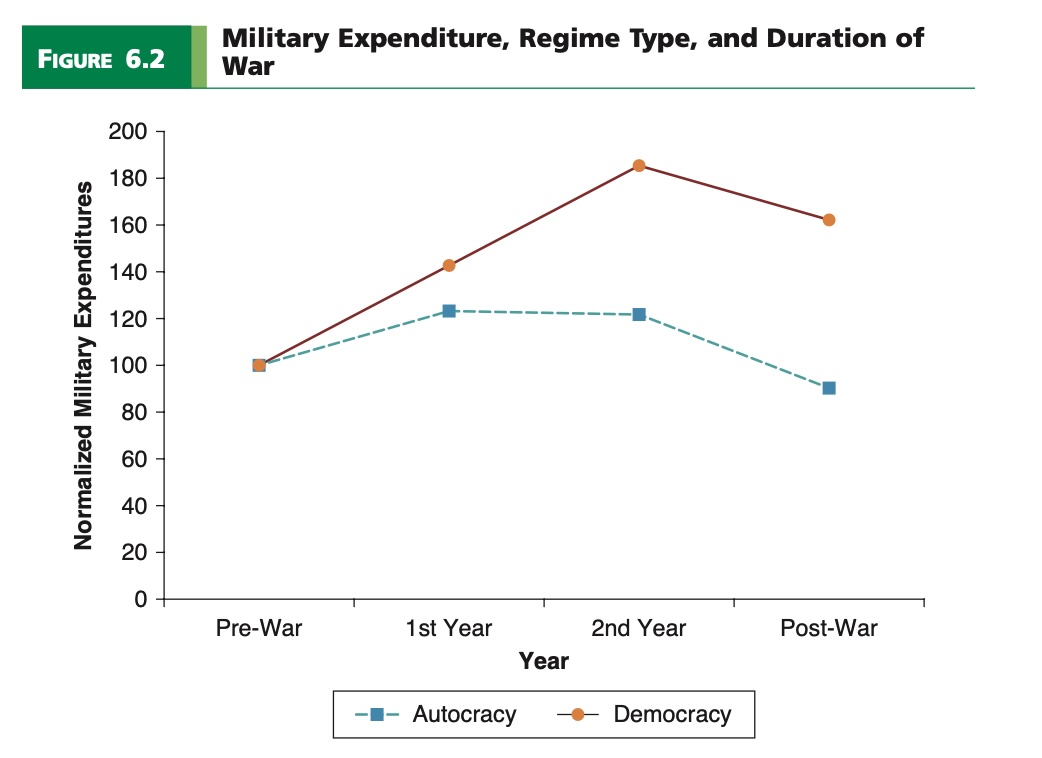
\includegraphics[width=1\textwidth]{images/military_expenditure_regime_type_duration_war.jpg}
    \captionof{figure}{\label{fig:fig9_military_expenditure_regime_type_duration_war.jpg}%\textit{\parencite[Fig.\(\backsim\)1]{cranmerWhatCanWe2017}}
    }
\end{center}

\textbf{This figure shows that democrats facing a prolonged war increase their effort tremendously.}

Figure 6.2 also shows us what happens after the war is over. Democrats cut back modestly on military spending, while autocrats return to their baseline level or even below.
The systematic evidence supports the war effort logic

\subsection{War Effort, War Loss, and Leader Deposition}
Since victorious democrats are more likely to depose and replace vanquished rivals than are victorious autocrats, small-coalition dictators must be especially nervous about defeat at the hands of a democrat.

